\documentclass[a4paper,11pt]{article}
\usepackage{a4wide}%

\usepackage{fullpage}%
\usepackage[T1]{fontenc}%
\usepackage[utf8]{inputenc}%
\usepackage[main=francais,english]{babel}%

\usepackage{graphicx}%
\usepackage{xspace}%
\usepackage{float}

\usepackage{url} \urlstyle{sf}%
\DeclareUrlCommand\email{\urlstyle{sf}}%

\usepackage{mathpazo}%
\let\bfseriesaux=\bfseries%
\renewcommand{\bfseries}{\sffamily\bfseriesaux}

\newenvironment{keywords}%
{\description\item[Mots-clés.]}%
{\enddescription}


\newenvironment{remarque}%
{\description\item[Remarque.]\sl}%
{\enddescription}

\font\manual=manfnt
\newcommand{\dbend}{{\manual\char127}}

\newenvironment{attention}%
{\description\item[\dbend]\sl}%
{\enddescription}

\usepackage{listings}%

\lstset{%
  basicstyle=\sffamily,%
  columns=fullflexible,%
  language=c,%
  frame=lb,%
  frameround=fftf,%
}%

\lstMakeShortInline{|}

\parskip=0.3\baselineskip

\sloppy

%opening
\title{PROG2: Inversion de matrices}
\author{Rémi Hutin \and Rémy Sun}
\date{28 février 2016}


\begin{document}

\maketitle

\begin{abstract}
  L'inversion de matrice est un problème algorithmique posant certaines difficultés, comme les erreurs de calculs dans des cas pathologiques comme les matrices de Hilbert.
  De plus, le calcul du déterminant par la méthode de Kramer engendre le calcul de beaucoup de sous-matrices, ce qui cause de gros problèmes de mémoire pour l'implémentation naïve des matrices.

  Nous proposons dans cet article une construction alternative du type matrice permettant d'éviter la construction explicite des sous-matrices et exposerons les diverses difficultées soulevées par cette construction.
  \begin{keywords}
    Matrice; Inversion; Sous-matrices implicites
  \end{keywords}
\end{abstract}

\section{Implémentation de matrices}

\subsection{Définition}

On définit une classe \texttt{Matrix} possédant trois champs privés : \texttt{size\_i} contenant le nombre de lignes de la matrice, \texttt{size\_j} donnant le nombre de colonnes et
 \texttt{contents} correspondant aux valeurs de la matrice.

Le champ  \texttt{contents}  contient un double vecteur de \texttt{scalar\_t} représentant la matrice des valeurs.

\subsection{Méthodes et fonctions}

On définit les méthodes publiques suivantes:

\begin{itemize}
\item \texttt{get\_size\_i} et \texttt{get\_size\_j} permettent de consulter la valeur de \texttt{size\_i} et \texttt{size\_j}
\item \texttt{set(j,j,x)} permet de remplacer la valeur d'indice \texttt{(i,j)} dans la matrice par \texttt{x}. \texttt{get(i,j)} permet de consulter la valeur d'indice\texttt{(i,j)} dans la matrice. \texttt{print()} affiche la matrice dans le terminal en formatant correctement l'affichage.
\end{itemize}

De plus, on définit les fonctions suivantes:

\begin{itemize}
\item Des opérateurs \texttt{+},\texttt{-} qui effectuent la somme et la différence de deux matrices en effectuant un simple parcours de la matrice. Un opérateur \texttt{*} qui possède deux sens différents: si le premier paramètre est un \texttt{scalar\_t} alors on effectue juste la mutltiplication scalaire de la matrice. Si c'est une matrice, on effectue une multiplication matricielle.
\item Une fonction \texttt{transpose} qui crée la matrice transposée par simple parcours des valeurs de la matrice. Une fonction \texttt{Id} qui crée une matrice identité.
\item Une fonction \texttt{submatrix} qui crée explicitement la sous-matrice obtenue en retirant une ligne et colonne spécifiée. (\textbf{voir section 1.3})
\item Une fonction \texttt{determinant} récursive qui calcule le déterminant par utilisation du développement par ligne.
\item Une fonction \texttt{inverse} qui calcule la matrice inverse.
\end{itemize}

\subsection{Extraction de sous-matrice}

Il est nécessaire d'extraire une sous-matrice en retirant la ligne d'indice $a$ et la colonne d'indice $b$. 

Ceci est fait en créant une matrice carrée de taille (\texttt{size\_i-1}, \texttt{size\_j-1}), qu'on remplit en parcourant la matrice d'origine.

\subsection{Erreurs de calcul d'inverse}

Le calcul de l'inverse est sujet à des erreurs d'arrondis. De fait, il est nécessaire de mesurer l'erreur commise.

La mesure de l'erreur a été définie par la norme infinie de $M\times M' - I_n$ ou $M'\times M - I_n$ où $M'$ est la matrice inverse calculée par le programme proposé.

Pour $n \in \{2;3;\dots;7\}$ on génère les matrices de Hilbert de taille $n$ et on calcule l'erreur commise. (Voir figure 1) L'étude du cas des matrices de Hilbert est intéressante car c'est un exemple de matrices mal conditionnées pour la méthode de Kramer.


\begin{figure}
  \centering
  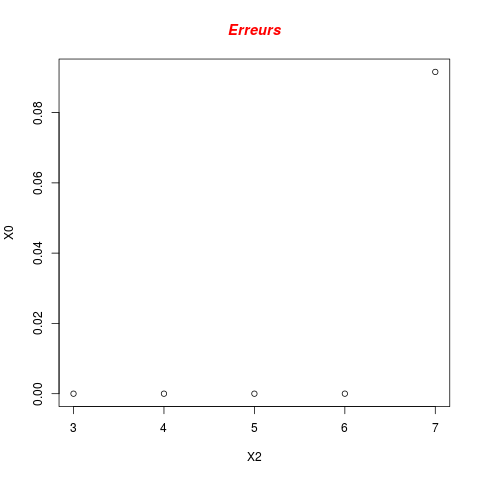
\includegraphics[scale=0.5]{Error.png}
  \caption{Erreurs pour les matrices de Hilbert}
  \label{fig:phd}
\end{figure}

\section{Optimisation: implémentation des sous-matrices}


Jusqu'à maintenant, chaque matrice possédait un champ \texttt{contents} correspondant à un double vecteur de valeurs.

Ce double vecteur est propre à chaque matrice déclarée. Ainsi, à chaque sous-matrice déclarée, on explicite à chaque fois la sous-matrice de valeurs, en copiant les valeurs de la matrice dans la mémoire. Cela prend énormément de place en mémoire.

Nous allons maintenant présenter une façon d'éviter à avoir à expliciter les sous-matrices.

\subsection{Définition de matrices par vecteurs de bits d'activité}

Nous passons contents en attribut \texttt{static} de la classe \texttt{Matrix}: toutes les matrices partagent le même champ \texttt{contents}.

L'idée est de faire de \texttt{contents} un triple vecteur (c'est-à-dire un vecteur de matrices) tel que la première coordonnée repère l'index de la matrice considérée. (Voir figure 2)

\begin{figure}
  \centering
  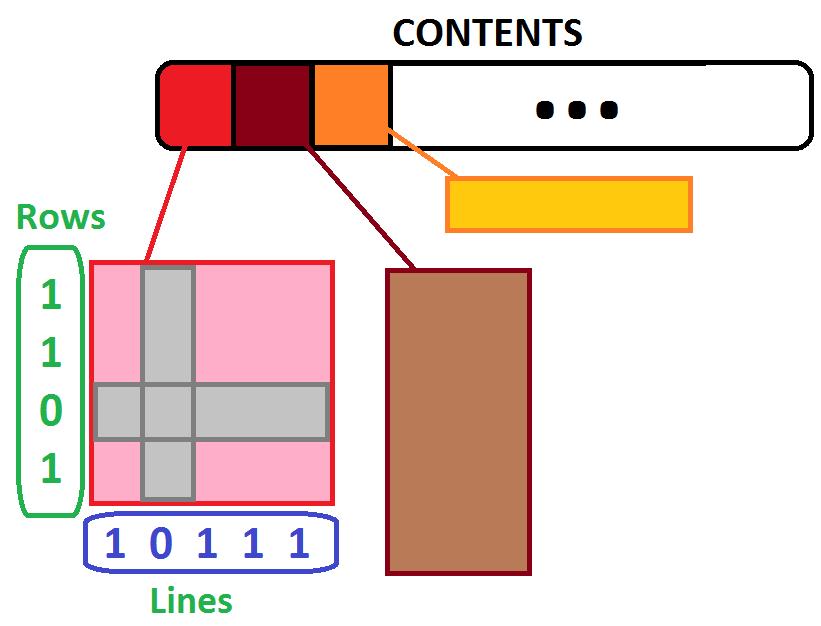
\includegraphics[scale=0.5]{matimpli.png}
  \caption{Nouvelle organisation du champ contents}
  \label{fig:phd}
\end{figure}

Ainsi, à chaque fois qu'une nouvelle matrice (à part entière) est créée, on ajoute sa matrice de valeurs au vecteur \texttt{contents}. Le champ \texttt{index} de la matrice repère son indice dans \texttt{contents}.

De plus, pour chaque matrice, on crée deux vecteurs \texttt{lines} et \texttt{rows} qui repèrent quelles lignes et colonnes de la matrice sont ``actives''.


\subsection{Redéfinition des méthodes de base}

La plus grosse difficulté posée par cette construction est que l'accès à la valeur \texttt{(i,j)} de la matrice n'est plus direct: certaines lignes et colonnes sont ``désactivées''. 
Pour remédier à cela, on crée une fonction \texttt{find\_nth} qui retourne la n-ième valeur non nulle d'un vecteur de booléens.

A partir de là, il devient très simple de redéfinir toutes les méthodes de base de Matrix en prenant soin de se rappeler que \texttt{contents} est maintenant un triple vecteur.

\subsection{Copie de matrice}

Notre surcharge du constructeur de copie de la classe \texttt{Matrix}  ne copie pas toutes les valeurs de la matrice: il ne rajoute rien au vecteur \texttt{contents}. Il se contente de copier l'\texttt{index} de la matrice dont il est copié (ainsi que ses autres champs privés).

\subsection{Création de sous-matrices}

La création de sous-matrice devient très simple: on crée une copie de la matrice en question, puis on modifie les vecteurs \texttt{rows} et \texttt{lines} pour refléter le changement dans la matrice considérée.

Cela présente le grand avantage de ne pas explicitement créer un nouveau double vecteur de valeurs pour la sous-matrice. Sachant que la fonction determinant fait $n!$ appels à la fonction submatrix les économies en temps (et mémoire) sont substantielles.


\subsection{Comparaisons avec l'ancienne méthode}

Nous avons annoncé à la partie précédente que cette nouvelle façon de procéder permet de faire des économies en temps de calcul.

Pour vérifier cette affirmation, on a effectué l'expérience suivante:

Pour $n \in \{2;3;\dots;8\}$ on génère des matrices aléatoires de taille $n$ et on compare les temps d'exécution de l'ancienne méthode et de la nouvelle.


\begin{figure}
  \centering
  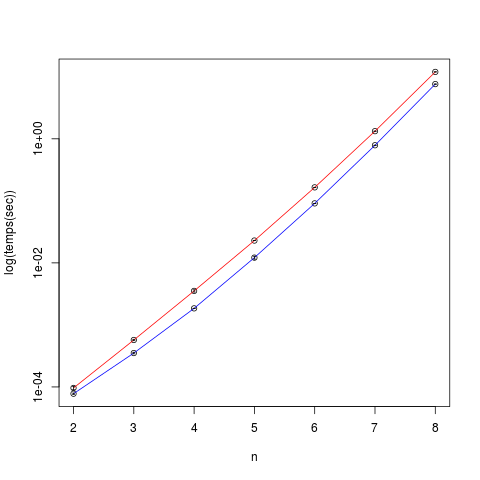
\includegraphics[scale=0.5]{Comparaison.png}
  \caption{Comparaison des deux méthodesde l'ancienne méthode (rouge) et de la nouvelle (bleu) avec barres d'écart-type}
  \label{fig:phd}
\end{figure}


\subsection{Fuites de mémoire}

Il est important de remarquer que notre implémentation à l'aide d'un vecteur statique n'est pas sans poser des problèmes de fuites mémoires.
En effet, la déclaration de nouvelles matrices dans une boucle peut causer une augmentation définitive du champ static \texttt{contents}.

\begin{lstlisting}
for (i=0; i < 10000; i++)
    Matrix M(10,10)
\end{lstlisting}


Avec l'ancienne implémentation, \texttt{M} est déclarée puis oubliée à chaque tour de boucle.

Avec notre nouvelle implémentation à l'aide du type \texttt{static}, toutes les matrices demeurent stockées dans \texttt{contents}.

Il est donc nécessaire de définir un moyen d'effacer des matrices de \texttt{contents} pour au moins minimiser les coûts en mémoire.

On a créé un vecteur \texttt{count} qui repère pour chaque matrice de valeurs stockée le nombre de matrices s'y référant. A chaque fois qu'une matrice ou sous-matrice est créée, on incrémente le compteur correspondant. On surcharge le destructeur pour qu'il décrémente ce compteur. Si le compteur atteint 0, on libère l'espace dans le vecteur.

\begin{remarque}
Avec l'ancienne implémentation, la boucle proposée plus haut occupe plusieurs méga-octets de mémoire, alors que la nouvelle implémentation n'occupe que quelques kilo-octets.
\end{remarque}

\subsection{Insuffisances}

Cette méthode présente cependant un gros inconvénient: les sous-matrices ainsi déclarées ont un contenu directement lié à celui des matrices mères. Si on modifie leur contenu, on modifie aussi celui de la matrice mère, et vice-versa.

Cela ne pose pas de problème dans le projet proposé puisque l'application qui en est faite agit en place sur le problème et ne modifie pas les valeurs des matrices.

\section*{Conclusion}

Nous avons étudié la construction naturelle des matrices et avons exposé le problème posé par les cas pathologiques de la méthode de Kramer.

Afin d'éviter l'éceuil de l'accumulation de sous-matrices explicites, nous avons défini un nouveau type de matrices composé de deux vecteurs d'activités donnant les lignes et colonnes actives référant à une matrice \texttt{static} commune à toutes les matrices de la classe.

Les gains en temps de calcul sont confirmés par l'expérience menée, et une adaptation du destructeur de la classe permet d'économiser un espace mémoire considérable. 

\end{document}
